\section{Обзор основных понятий и законов классической механики}
\subsection{Механика как часть теоретической физики}
Общая (экспериментальная) физика основана на принципе индукции и поставляет теоретической физике математические модели (физические законы). Теоретическая физика использует дедукцию, и возвращает общей физике предсказания результатов экспериментов.

\begin{dfn} Механика --- наука о движении материальных объектов в пространстве и времени. \end{dfn}
Откажемся от определения, в котором сложно объяснить слова в правой части, и будем перечислять...
\begin{enumerate}
\item Пространство и время независимы.
\item Пространство трёхмерно, евклидово, однородно, изотропно.
\item Время однородно, однонаправленно (?).
\end{enumerate}
С точки зрения современной физики эти положения неверны, но это представления классической физики. А как сделать их более корректными?
\begin{enumerate}
\item СТО $v \ll c$.
\item КМ $\Delta l \gg \frac{\hbar}{p}$ --- длина волны де Бройля.
\item ОТО $m \varphi \ll mc^2$, $\varphi$ --- потенциал.
\item ВВ $t \gg t_{BB}$.
\end{enumerate}

\begin{dfn}
Материальная точка --- тело, размерами которого при рассмотрении данного класса движение модно пренебречь.
\end{dfn}
\begin{dfn}
Абсолютно твёрдое тело --- набор материальных точек, расстояния между которыми не изменяются.
\end{dfn}

\begin{task}[Задача Кэлли (?)] \index{Задача Кэлли}Какое минимальное количество связей между материальными точками необходимо установить, чтобы их система обрела жёсткость? \end{task}

\subsection{Механика системы материальных точек}
\begin{equation*}
\vb{r}(t) = \{x(t), y(t), z(t) \}; \thickspace \mathop{\{\vb{r}_i(t)\}}\limits_{i = \overline{1{,}N}}
\end{equation*}  

\subsubsection{Кинематика материальной точки.}
$\vb{r}(t)$ --- закон движения (иногда знаем траекторию и положение точки для любого момента времени). 
\begin{align*}
\vb{r} &= r \vb{e}_r = \sqrt{x^2 + y^2 + z^2} \vb{e}_r, \\
\vb{e}_r &= \frac{\vb{r}}{r} = \left\{ \frac{x}{\sqrt{x^2 + y^2 + z^2}}, \frac{y}{\sqrt{x^2 + y^2 + z^2}}, \frac{z}{\sqrt{x^2 + y^2 + z^2}} \right\};\\
\vb{v} &= \dv{\vb{r}}{t} = \left\{\dot x, \dot y, \dot z\right\},\\
\vb{v} &= v \vb*{\tau}.
\end{align*}

\paragraph{Криволинейные координаты.}\index{Координаты! криволинейные}
\begin{align*}
q &= (q_1, q_2, q_3), x =X(q, t), y = Y(q, t), z =Z(q, t) \Rightarrow \\
q(t) &\Rightarrow \vb{r}(t) = \vb{r}{\vb{q}(t), t} = \left\{X(q(t), t), Y(q(t), t), Z(q(t), t)\right\}; \\
\vb{v}(t) &= \dv{\vb{r}}{t} = \sum \pdv{\vb{r}}{q_i} \dot q_i + \pdv{\vb{r}}{t}; \\
\vb{v}_i &= \left\{\pdv{X}{q_i} \dot q_i, \pdv{Y}{q_i} \dot q_i, \pdv{Z}{q_i} \dot q_i \right\}.
\end{align*}

\begin{equation*}
\vb{v} = \sum v_i \vb{e}_i; (e_i, e_j) = \delta_{ij} \Rightarrow v^2 = v_1^2 + v_2^2 + v_3^2
\end{equation*}

\begin{ex}[Цилиндрические координаты] \index{Координаты! цилиндрические} Пусть $q = (\varphi, \rho, z),$ и
\begin{equation*}
\begin{cases}
x = \rho \cos \varphi   \\
y = \rho \sin \varphi \\
z,
\end{cases}
\end{equation*}
тогда
\begin{equation*}
\vb{v} = \dv{t} \left\{\rho \cos \varphi, \rho \sin \varphi, z \right\} \Rightarrow
\end{equation*}
\begin{equation*}
\begin{cases}
\vb{v}_{\varphi} = \rho \dot \varphi \underbrace{\{-\sin \varphi, \cos \varphi, 0\}}_{\vb{e}_\varphi} \\
\vb{v}_\rho = \dot \rho \underbrace{\{\cos \varphi, \sin \varphi, 0\}}_{\vb{e}_\rho} \\
\vb{v}_z = \dot z \{0, 0, 1\},
\end{cases}
\end{equation*}
значит, 
\begin{equation*}
(\vb{e}_\rho, \vb{e}_\varphi) = 0.
\end{equation*}
\end{ex}

\paragraph{Ускорение.}\index{Ускорение}\index{Ускорение}
\begin{align*}
\vb{a} & \eqdef \dv{\vb{v}}{t} = \dv[2]{\vb{r}}{t} = \left\{\ddot{x}, \ddot{y}, \ddot{z} \right\} \\
\vb{a} &= \dv{t} (v \vb*{\tau}) = \dot{v} \vb*{\tau} + \underbrace{v \dot{\vb*{\tau}}}_{= \frac{v^2}{R} \vb{n}} \\
\vb{n} &= \frac{\dot{\vb{r}}}{\dot{\vb*{\tau}}}\\
\abs{\dot{\vb*{\tau}}} &= \frac{v}{R}\\
[\vb*{\tau}, \vb{n}] &= \vb{b} \thickspace \text{--- бинормаль --- по ней не может быть направлено ускорение.}
\end{align*}


\subsubsection{Основные постулаты ньютоновской механики.}
Сразу отметим, что количество точек в системе может быть бесконечным, или даже несчётным.

\begin{enumerate}
\item[0.] Пространство $+$ Время классические (однонаправленность времени не учитываем).
\item Первый закон Ньютона: \index{Законы Ньютона! первый} существуют инерциальные системы отсчёта, в которых изолированная точка движется равномерно и прямолинейно.

Добавим принцип относительности Галилея, чтобы не возникало выделенных направлений из-за введения системы отсчёта: законы движения инвариантны относительно преобразования Галилея в замкнутой системе. Преобразование Галилея\index{Преобразование Галилея}:
\begin{equation}
\begin{cases}
t = t'\\
\vb{r'} = \vb{r} + \vb{u}t, \qquad \vb{u} = const.
\end{cases}
\label{Galilean_tr}
\end{equation}
Система \eqref{Galilean_tr} порождает бесконечный класс инерциальных систем, и однородность восстанавливается.

\item Второй закон Ньютона. \index{Законы Ньютона! второй} Принцип детерминизма Ньютона <<сидит>> в порядке дифференциальных уравнений для описания динамики системы.
\begin{equation*}
\Ddot{\vb{r}}_i = \vb{f}_i (\vb{r}_1, \dots, \vb{r}_N, \vb{v}_1, \dots, \vb{v}_N, t) 
\end{equation*}
$6N$ свободных констант --- по две на каждую степень свободы.
\begin{equation*}
\begin{cases}
\vb{r}_i (t_0) = {\vb{r}_i}_0\\
\vb{v}_i (t_0) = {\vb{v}_i}_0,
\end{cases}
\end{equation*}
существует, правда, множество меры нуль всяких исключений: диссипативные состояния равновесия, например.

Второй закон Ньютона:
\begin{equation}
m_i \ddot{\vb{r}}_i = \vb{F}_i \left(\{\vb{r}_i\}, \{\dot{\vb{r}}_i\}, t\right).
\label{Newton's_2nd_law}
\end{equation}
Отметим, что уравнение \eqref{Newton's_2nd_law} работает в инерциальных системах отсчёта, $m_i$ --- характеристика материальной точки, не зависящая от движения.

Экспериментальный способ измерения:
\begin{equation*}
\begin{cases}
m_1 a_1 = F\\
m_2 a_2 = F
\end{cases}
\Rightarrow \; \frac{m_1}{m_2} = \frac{a_2}{a_1}, \qquad
\begin{cases}
ma_1 = F_1\\
ma_2 = F_2
\end{cases}
\Rightarrow \; \frac{F_1}{F_2} = \frac{a_1}{a_2}.
\end{equation*}
\paragraph{Импульс.}
\begin{align*}
\vb{p}_i & \eqdef m_i \vb{v}_i && \text{--- импульс,}\\
\vb{M}_i & \eqdef m_i [\vb{r}_i, \vb{v}_i] && \text{--- момент импульса,}\\
\vb{N}_i & \eqdef [\vb{r}_i, \vb{F}_i] && \text{--- момент силы.}\index{Момент! силы} \index{Момент! импульса}
\end{align*}

\begin{cex}
Могут быть патологические случаи.
$m(t)$ --- ракета и реактивная сила или, например, тележка с тающим льдом: включаем массу в систему --- система с сохраняющейся массой, а потом смотрим на динамику подсистем. $\vb{F}$ может зависеть от разных других вещей, когда мы пытаемся описать механическим немеханические явления: $m(\dot{\vb{r}})$ --- квазиклассические частицы в твёрдом теле, тела в СТО, $m(\ddot{\vb{r}})$ --- присоединённая масса в гидродинамике, $F(\dddot{\vb{r}})$~--- радиационное трение~--- электрон летает вокруг ядра по боровской  орбите, излучает электромагнитные волны как любой движущийся заряд, теряя таким образом энергию, и падает на ядро, нарушается принцип детерминизма Ньютона --- пытаемся описать электромагнитную задачу механическим языком.
\end{cex}

\item
Третий закон Ньютона. \index{Законы Ньютона! третий}Чтобы его определить, придётся все силы разбить на внутренние и внешние.
\begin{equation*}
\vb{F}_i = \vb{F}_i^{(e)} (t, \vb{r}_i) + \sum \vb{F}_{ij}^{(i)} (t, \vb{r}_i, \vb{r}_j), 
\end{equation*}
внешняя сила может зависеть только от координаты точки (и времени), а все оставшиеся силы~--- внутренние. Для <<всех оставшихся>>  предположили, что каждая из точек действует на $i$-ю точку независимо от всех остальных. И обрываем ряд, то есть считаем, что силы, в которой есть $\vb{r}_i, \vb{r}_j$ и $\vb{r}_k$ уже нет~--- приближение парных взаимодействий, и третий закон Ньютона справедлив только при  его применении. Формулировка третьего закона Ньютона \index{Законы Ньютона! третий}:

\begin{figure}[h]\centering
\def\svgwidth{9cm}
\input{pic3.pdf_tex}
\end{figure}
                                                                      
\begin{equation}
\begin{cases}
\vb{F}_{ij}^{(i)} + \vb{F}_{ji}^{(i)} = 0 \label{3d_N's-law}\\
[\vb*{\rho}_{ij}, \vb{F}_{ij}] = 0 
\end{cases}
\end{equation}


\begin{cex}
Третий закон Ньютона справедлив только для объектов, которые являются материальными точками, но существуют объекты нулевого размера, не являющиеся материальными точками: например, электрический диполь, у которого есть вращающий момент, который может ещё и энергию забирать...
\end{cex}
\begin{cns}


\begin{enumerate}
\item \begin{equation*}
 \vb{F} = \sum \limits_{i = 1}^N \vb{F}_i^{(e)} = \vb{F}^{(e)} \Rightarrow \left( \sum m_i \right) \cdot \vb{\ddot{R}} = \vb{F} = \vb{F}^{(e)}, \vb{R} = \frac{\sum m_i \vb{r}_i}{\sum m_i},\index{Центр масс}
\end{equation*}
то есть центр масс системы материальных точек  с попарным взаимодействием движется так же, как одна точка с суммарной массой системы в поле равнодействующей всех внешних сил.
\begin{ex}
Центр масс двигавшегося по параболе и разорвавшегося в некоторой точке снаряда продолжит движение по параболе.
\end{ex}
\begin{cex}
У Карлсона, летящего по параболе, раскрылся парашют...
\end{cex} 
\item \begin{equation*}
\vb{N} = \sum \vb{N}_i = \sum \vb{N}_i^{(e)},
\end{equation*}
то есть суммарный момент сил, действующих на систему с попарным взаимодействием, равен суммарному моменту внешних сил. Как это можно доказать?
\begin{equation}
[\vphantom{\vb{F}_{j}}\vb{r}_i, \vb{F}_{ij}] + [\vphantom{\vb{F}_{j}}\vb{r}_j, \vb{F}_{ji}] = [\vphantom{\vb{F}_{j}}\vb{r}_i - \vb{r}_j, \vb{F}_{ij}] = 0, \label{ftr_3d_N's-law}
\end{equation}
то есть сначала воспользовались первой часть третьего закона Ньютона \eqref{3d_N's-law}, чтобы поменять знак, а потом --- второй, чтобы приравнять к нулю.
\end{enumerate}
\end{cns}
\end{enumerate}
\newpage
\subsubsection{Законы сохранения в механике Ньютона.}
\subparagraph{Закон сохранения импульса.} \index{Закон сохранения! импульса}

\begin{gather*}
\vb{p} \eqdef \sum m_i \vb{v}_i \Rightarrow\\
\dot{\vb{p}} = \vb{F} = \vb{F}^{(e)},
\end{gather*}
первый переход осуществлён в силу II закона Ньютона, второй --- III закона Ньютона.
\begin{equation*}
\vb{p} = const \Leftarrow \sum \vb{F}_i^{(e)} = 0,
\end{equation*}
согласно III закону Ньютона.

\subparagraph{Закон сохранения момента импульса.} \index{Закон сохранения! момента импульса}
\begin{gather*}
\vb{M} \eqdef \sum m_i [\vb{r}_i, \vb{v}_i];\\
\dot{\vb{M}} = \sum m_i \bigl\{ [\vb{r}_i, \dot{\vb{v}}_i] + [\dot{\vb{r}_i}, \vb{v}] \bigr\} = \vb{N} = \vb{N}^{(e)};\\
\begin{cases}
\sum \vb{N}_i^{(e)} = 0,\\
\text{III закон Ньютона}
\end{cases}
\Rightarrow \vb{M} = const
\end{gather*}
\subparagraph{Закон сохранения энергии.} \index{Закон сохранения! энергии! для одной материальной точки}
\begin{gather*}
m \ddot{\vb{r}} = \vb{F} \qquad |\cdot \vb{v} \Rightarrow\\
m \vb{v} \dv{\vb{v}}{t} = m \left( v_x \dot{v}_x + v_y \dot{v}_y + v_z \dot{v}_z \right) = \frac{m}{2} \cdot2 \dv{t} \left( v_x^2 + v_y^2 + v_z^2 \right) = \dv{T}{t} \Rightarrow\\
T = \frac{mv^2}{2} 
\end{gather*}
\begin{figure}[h]\centering
\def\svgwidth{7cm}
%LaTeX with PSTricks extensions
%%Creator: inkscape 0.92.3
%%Please note this file requires PSTricks extensions
\psset{xunit=.5pt,yunit=.5pt,runit=.5pt}
\begin{pspicture}(793.7007874,1122.51968504)
{
\newrgbcolor{curcolor}{0 0 0}
\pscustom[linewidth=0.60732901,linecolor=curcolor]
{
\newpath
\moveto(189.77664889,195.44104651)
\curveto(192.96828537,207.40297161)(194.93820634,223.75863739)(211.72998819,227.53531623)
\curveto(244.2983589,234.86035102)(277.71617316,209.194393)(305.94640956,217.66014962)
\curveto(346.45433384,229.80781159)(332.4532171,287.32880867)(369.0622661,298.30724928)
\curveto(405.39902765,309.20404491)(441.05372138,273.90866077)(482.48784121,292.54674993)
\curveto(496.69834581,298.93896367)(506.39595921,359.32339155)(521.82091916,374.01676563)
}
}
{
\newrgbcolor{curcolor}{0 0 0}
\pscustom[linestyle=none,fillstyle=solid,fillcolor=curcolor]
{
\newpath
\moveto(190.06957919,196.53891914)
\curveto(190.75695096,196.39047927)(191.18090692,195.7681217)(191.01590944,195.14972814)
\curveto(190.85091197,194.53133459)(190.15913402,194.14992289)(189.47176225,194.29836276)
\curveto(188.78439048,194.44680263)(188.36043453,195.0691602)(188.525432,195.68755376)
\curveto(188.69042948,196.30594731)(189.38220742,196.68735901)(190.06957919,196.53891914)
\closepath
}
}
{
\newrgbcolor{curcolor}{0 0 0}
\pscustom[linewidth=0.32390881,linecolor=curcolor]
{
\newpath
\moveto(190.06957919,196.53891914)
\curveto(190.75695096,196.39047927)(191.18090692,195.7681217)(191.01590944,195.14972814)
\curveto(190.85091197,194.53133459)(190.15913402,194.14992289)(189.47176225,194.29836276)
\curveto(188.78439048,194.44680263)(188.36043453,195.0691602)(188.525432,195.68755376)
\curveto(188.69042948,196.30594731)(189.38220742,196.68735901)(190.06957919,196.53891914)
\closepath
}
}
{
\newrgbcolor{curcolor}{0 0 0}
\pscustom[linestyle=none,fillstyle=solid,fillcolor=curcolor]
{
\newpath
\moveto(522.6826305,374.83760712)
\curveto(523.19655466,374.40094243)(523.21972735,373.67130608)(522.73435524,373.20895454)
\curveto(522.24898314,372.74660301)(521.43796009,372.72575572)(520.92403593,373.16242041)
\curveto(520.41011176,373.5990851)(520.38693907,374.32872145)(520.87231118,374.79107298)
\curveto(521.35768328,375.25342451)(522.16870633,375.2742718)(522.6826305,374.83760712)
\closepath
}
}
{
\newrgbcolor{curcolor}{0 0 0}
\pscustom[linewidth=0.32390881,linecolor=curcolor]
{
\newpath
\moveto(522.6826305,374.83760712)
\curveto(523.19655466,374.40094243)(523.21972735,373.67130608)(522.73435524,373.20895454)
\curveto(522.24898314,372.74660301)(521.43796009,372.72575572)(520.92403593,373.16242041)
\curveto(520.41011176,373.5990851)(520.38693907,374.32872145)(520.87231118,374.79107298)
\curveto(521.35768328,375.25342451)(522.16870633,375.2742718)(522.6826305,374.83760712)
\closepath
}
}
{
\newrgbcolor{curcolor}{0 0 0}
\pscustom[linestyle=none,fillstyle=solid,fillcolor=curcolor]
{
\newpath
\moveto(175.56272854,169.83544104)
\lineto(174.31213131,169.83544104)
\lineto(174.29962534,173.22198888)
\curveto(173.42420727,173.2369902)(172.54878921,173.32699811)(171.67337115,173.49201263)
\curveto(170.79795309,173.6645278)(169.91836637,173.91955023)(169.03461099,174.25707991)
\lineto(169.03461099,176.28225802)
\curveto(169.88501711,175.8022158)(170.74376054,175.43843381)(171.61084129,175.19091204)
\curveto(172.48625935,174.95089093)(173.38668936,174.82713005)(174.31213131,174.81962939)
\lineto(174.31213131,179.9500806)
\curveto(172.46958472,180.22010435)(171.12727703,180.67764459)(170.28520822,181.32270132)
\curveto(169.45147674,181.96775805)(169.03461099,182.85283589)(169.03461099,183.97793484)
\curveto(169.03461099,185.20054237)(169.48899465,186.16437713)(170.39776198,186.86943914)
\curveto(171.3065293,187.57450115)(172.61131907,187.97953677)(174.31213131,188.08454601)
\lineto(174.31213131,190.72852854)
\lineto(175.56272854,190.72852854)
\lineto(175.56272854,188.11829898)
\curveto(176.33809882,188.08829634)(177.08845716,188.01328974)(177.81380356,187.89327919)
\curveto(178.53914995,187.78076929)(179.24782171,187.62325544)(179.93981885,187.42073763)
\lineto(179.93981885,185.45181447)
\curveto(179.24782171,185.76684217)(178.53498129,186.01061361)(177.80129758,186.18312878)
\curveto(177.07595119,186.35564395)(176.32976151,186.45690286)(175.56272854,186.4869055)
\lineto(175.56272854,181.68273298)
\curveto(177.45529902,181.42020989)(178.8476306,180.95141866)(179.73972329,180.27635929)
\curveto(180.63181598,179.60129992)(181.07786233,178.67871879)(181.07786233,177.50861588)
\curveto(181.07786233,176.24100439)(180.60263538,175.23966633)(179.65218149,174.50460168)
\curveto(178.71006491,173.77703769)(177.34691392,173.35700075)(175.56272854,173.24449086)
\closepath
\moveto(174.31213131,181.88525079)
\lineto(174.31213131,186.49815649)
\curveto(173.34500278,186.40064791)(172.60715042,186.15312614)(172.09857421,185.75559118)
\curveto(171.589998,185.35805622)(171.3357099,184.82925971)(171.3357099,184.16920166)
\curveto(171.3357099,183.52414493)(171.56915472,183.02160073)(172.03604435,182.66156907)
\curveto(172.5112713,182.3015374)(173.26996695,182.04276465)(174.31213131,181.88525079)
\closepath
\moveto(175.56272854,179.72506081)
\lineto(175.56272854,174.85338236)
\curveto(176.62156753,174.98089357)(177.4177811,175.25091732)(177.95136925,175.6634536)
\curveto(178.49329472,176.07598988)(178.76425745,176.61978771)(178.76425745,177.29484708)
\curveto(178.76425745,177.95490513)(178.50580069,178.4799513)(177.98888717,178.86998561)
\curveto(177.48031096,179.26001991)(176.67159142,179.54504498)(175.56272854,179.72506081)
\closepath
}
}
{
\newrgbcolor{curcolor}{0 0 0}
\pscustom[linestyle=none,fillstyle=solid,fillcolor=curcolor]
{
\newpath
\moveto(186.39290132,175.13465709)
\lineto(190.51987218,175.13465709)
\lineto(190.51987218,187.94953413)
\lineto(186.03022812,187.13946289)
\lineto(186.03022812,189.20964496)
\lineto(190.49486024,190.0197162)
\lineto(193.02106664,190.0197162)
\lineto(193.02106664,175.13465709)
\lineto(197.14803751,175.13465709)
\lineto(197.14803751,173.22198888)
\lineto(186.39290132,173.22198888)
\closepath
}
}
{
\newrgbcolor{curcolor}{0 0 0}
\pscustom[linestyle=none,fillstyle=solid,fillcolor=curcolor]
{
\newpath
\moveto(208.17830584,169.83544104)
\lineto(206.92770861,169.83544104)
\lineto(206.91520264,173.22198888)
\curveto(206.03978458,173.2369902)(205.16436652,173.32699811)(204.28894846,173.49201263)
\curveto(203.41353039,173.6645278)(202.53394367,173.91955023)(201.6501883,174.25707991)
\lineto(201.6501883,176.28225802)
\curveto(202.50059441,175.8022158)(203.35933785,175.43843381)(204.22641859,175.19091204)
\curveto(205.10183666,174.95089093)(206.00226666,174.82713005)(206.92770861,174.81962939)
\lineto(206.92770861,179.9500806)
\curveto(205.08516203,180.22010435)(203.74285433,180.67764459)(202.90078553,181.32270132)
\curveto(202.06705404,181.96775805)(201.6501883,182.85283589)(201.6501883,183.97793484)
\curveto(201.6501883,185.20054237)(202.10457196,186.16437713)(203.01333928,186.86943914)
\curveto(203.9221066,187.57450115)(205.22689638,187.97953677)(206.92770861,188.08454601)
\lineto(206.92770861,190.72852854)
\lineto(208.17830584,190.72852854)
\lineto(208.17830584,188.11829898)
\curveto(208.95367613,188.08829634)(209.70403447,188.01328974)(210.42938086,187.89327919)
\curveto(211.15472725,187.78076929)(211.86339902,187.62325544)(212.55539615,187.42073763)
\lineto(212.55539615,185.45181447)
\curveto(211.86339902,185.76684217)(211.1505586,186.01061361)(210.41687489,186.18312878)
\curveto(209.69152849,186.35564395)(208.94533881,186.45690286)(208.17830584,186.4869055)
\lineto(208.17830584,181.68273298)
\curveto(210.07087632,181.42020989)(211.46320791,180.95141866)(212.3553006,180.27635929)
\curveto(213.24739329,179.60129992)(213.69343963,178.67871879)(213.69343963,177.50861588)
\curveto(213.69343963,176.24100439)(213.21821269,175.23966633)(212.26775879,174.50460168)
\curveto(211.32564221,173.77703769)(209.96249123,173.35700075)(208.17830584,173.24449086)
\closepath
\moveto(206.92770861,181.88525079)
\lineto(206.92770861,186.49815649)
\curveto(205.96058009,186.40064791)(205.22272772,186.15312614)(204.71415151,185.75559118)
\curveto(204.20557531,185.35805622)(203.9512872,184.82925971)(203.9512872,184.16920166)
\curveto(203.9512872,183.52414493)(204.18473202,183.02160073)(204.65162165,182.66156907)
\curveto(205.1268486,182.3015374)(205.88554425,182.04276465)(206.92770861,181.88525079)
\closepath
\moveto(208.17830584,179.72506081)
\lineto(208.17830584,174.85338236)
\curveto(209.23714483,174.98089357)(210.0333584,175.25091732)(210.56694656,175.6634536)
\curveto(211.10887202,176.07598988)(211.37983476,176.61978771)(211.37983476,177.29484708)
\curveto(211.37983476,177.95490513)(211.121378,178.4799513)(210.60446447,178.86998561)
\curveto(210.09588827,179.26001991)(209.28716872,179.54504498)(208.17830584,179.72506081)
\closepath
}
}
{
\newrgbcolor{curcolor}{0 0 0}
\pscustom[linestyle=none,fillstyle=solid,fillcolor=curcolor]
{
\newpath
\moveto(537.79285197,356.64043999)
\lineto(536.54225474,356.64043999)
\lineto(536.52974877,360.02698783)
\curveto(535.65433071,360.04198915)(534.77891265,360.13199706)(533.90349458,360.29701158)
\curveto(533.02807652,360.46952675)(532.1484898,360.72454918)(531.26473443,361.06207886)
\lineto(531.26473443,363.08725697)
\curveto(532.11514054,362.60721475)(532.97388398,362.24343276)(533.84096472,361.99591099)
\curveto(534.71638278,361.75588988)(535.61681279,361.632129)(536.54225474,361.62462834)
\lineto(536.54225474,366.75507955)
\curveto(534.69970816,367.0251033)(533.35740046,367.48264354)(532.51533166,368.12770027)
\curveto(531.68160017,368.772757)(531.26473443,369.65783484)(531.26473443,370.78293379)
\curveto(531.26473443,372.00554132)(531.71911809,372.96937609)(532.62788541,373.67443809)
\curveto(533.53665273,374.3795001)(534.84144251,374.78453572)(536.54225474,374.88954496)
\lineto(536.54225474,377.53352749)
\lineto(537.79285197,377.53352749)
\lineto(537.79285197,374.92329793)
\curveto(538.56822226,374.89329529)(539.3185806,374.81828869)(540.04392699,374.69827814)
\curveto(540.76927338,374.58576824)(541.47794515,374.42825439)(542.16994228,374.22573658)
\lineto(542.16994228,372.25681342)
\curveto(541.47794515,372.57184112)(540.76510473,372.81561256)(540.03142102,372.98812773)
\curveto(539.30607462,373.16064291)(538.55988494,373.26190181)(537.79285197,373.29190445)
\lineto(537.79285197,368.48773193)
\curveto(539.68542245,368.22520885)(541.07775403,367.75641762)(541.96984673,367.08135825)
\curveto(542.86193942,366.40629888)(543.30798576,365.48371774)(543.30798576,364.31361483)
\curveto(543.30798576,363.04600335)(542.83275882,362.04466528)(541.88230492,361.30960063)
\curveto(540.94018834,360.58203664)(539.57703736,360.1619997)(537.79285197,360.04948981)
\closepath
\moveto(536.54225474,368.69024974)
\lineto(536.54225474,373.30315544)
\curveto(535.57512622,373.20564686)(534.83727385,372.9581251)(534.32869764,372.56059013)
\curveto(533.82012144,372.16305517)(533.56583333,371.63425866)(533.56583333,370.97420061)
\curveto(533.56583333,370.32914388)(533.79927815,369.82659968)(534.26616778,369.46656802)
\curveto(534.74139473,369.10653636)(535.50009038,368.8477636)(536.54225474,368.69024974)
\closepath
\moveto(537.79285197,366.53005976)
\lineto(537.79285197,361.65838131)
\curveto(538.85169096,361.78589252)(539.64790453,362.05591627)(540.18149269,362.46845255)
\curveto(540.72341815,362.88098883)(540.99438089,363.42478666)(540.99438089,364.09984603)
\curveto(540.99438089,364.75990408)(540.73592412,365.28495026)(540.2190106,365.67498456)
\curveto(539.71043439,366.06501886)(538.90171485,366.35004393)(537.79285197,366.53005976)
\closepath
}
}
{
\newrgbcolor{curcolor}{0 0 0}
\pscustom[linestyle=none,fillstyle=solid,fillcolor=curcolor]
{
\newpath
\moveto(550.3613549,361.93965604)
\lineto(559.17806538,361.93965604)
\lineto(559.17806538,360.02698783)
\lineto(547.32240363,360.02698783)
\lineto(547.32240363,361.93965604)
\curveto(548.28119484,362.83223454)(549.58598462,364.02858976)(551.23677297,365.5287217)
\curveto(552.89589863,367.03635429)(553.93806299,368.00768972)(554.36326604,368.44272798)
\curveto(555.17198559,369.26029988)(555.73475434,369.95036057)(556.05157231,370.51291004)
\curveto(556.37672759,371.08296018)(556.53930523,371.64175932)(556.53930523,372.18930748)
\curveto(556.53930523,373.08188598)(556.189138,373.80944997)(555.48880355,374.37199944)
\curveto(554.79680642,374.93454892)(553.89220775,375.21582366)(552.77500756,375.21582366)
\curveto(551.98296265,375.21582366)(551.1450625,375.09206277)(550.26130713,374.844541)
\curveto(549.38588906,374.59701923)(548.44794114,374.22198625)(547.44746336,373.71944205)
\lineto(547.44746336,376.01464391)
\curveto(548.46461577,376.38217623)(549.41506967,376.65970064)(550.29882504,376.84721713)
\curveto(551.18258042,377.03473362)(551.99129996,377.12849187)(552.72498367,377.12849187)
\curveto(554.65924072,377.12849187)(556.20164397,376.69345361)(557.35219343,375.82337709)
\curveto(558.50274288,374.95330057)(559.07801761,373.79069832)(559.07801761,372.33557034)
\curveto(559.07801761,371.64550965)(558.9321146,370.98920193)(558.64030858,370.36664718)
\curveto(558.35683987,369.75159309)(557.83575769,369.0240291)(557.07706204,368.18395522)
\curveto(556.86862916,367.96643609)(556.20581263,367.33638067)(555.08861244,366.29378898)
\curveto(553.97141225,365.25869795)(552.39565973,363.8073203)(550.3613549,361.93965604)
\closepath
}
}
{
\newrgbcolor{curcolor}{0 0 0}
\pscustom[linestyle=none,fillstyle=solid,fillcolor=curcolor]
{
\newpath
\moveto(570.40842928,356.64043999)
\lineto(569.15783205,356.64043999)
\lineto(569.14532607,360.02698783)
\curveto(568.26990801,360.04198915)(567.39448995,360.13199706)(566.51907189,360.29701158)
\curveto(565.64365383,360.46952675)(564.76406711,360.72454918)(563.88031173,361.06207886)
\lineto(563.88031173,363.08725697)
\curveto(564.73071785,362.60721475)(565.58946128,362.24343276)(566.45654203,361.99591099)
\curveto(567.33196009,361.75588988)(568.2323901,361.632129)(569.15783205,361.62462834)
\lineto(569.15783205,366.75507955)
\curveto(567.31528546,367.0251033)(565.97297776,367.48264354)(565.13090896,368.12770027)
\curveto(564.29717747,368.772757)(563.88031173,369.65783484)(563.88031173,370.78293379)
\curveto(563.88031173,372.00554132)(564.33469539,372.96937609)(565.24346271,373.67443809)
\curveto(566.15223003,374.3795001)(567.45701981,374.78453572)(569.15783205,374.88954496)
\lineto(569.15783205,377.53352749)
\lineto(570.40842928,377.53352749)
\lineto(570.40842928,374.92329793)
\curveto(571.18379956,374.89329529)(571.9341579,374.81828869)(572.65950429,374.69827814)
\curveto(573.38485069,374.58576824)(574.09352245,374.42825439)(574.78551959,374.22573658)
\lineto(574.78551959,372.25681342)
\curveto(574.09352245,372.57184112)(573.38068203,372.81561256)(572.64699832,372.98812773)
\curveto(571.92165193,373.16064291)(571.17546225,373.26190181)(570.40842928,373.29190445)
\lineto(570.40842928,368.48773193)
\curveto(572.30099975,368.22520885)(573.69333134,367.75641762)(574.58542403,367.08135825)
\curveto(575.47751672,366.40629888)(575.92356307,365.48371774)(575.92356307,364.31361483)
\curveto(575.92356307,363.04600335)(575.44833612,362.04466528)(574.49788222,361.30960063)
\curveto(573.55576564,360.58203664)(572.19261466,360.1619997)(570.40842928,360.04948981)
\closepath
\moveto(569.15783205,368.69024974)
\lineto(569.15783205,373.30315544)
\curveto(568.19070352,373.20564686)(567.45285115,372.9581251)(566.94427495,372.56059013)
\curveto(566.43569874,372.16305517)(566.18141064,371.63425866)(566.18141064,370.97420061)
\curveto(566.18141064,370.32914388)(566.41485545,369.82659968)(566.88174509,369.46656802)
\curveto(567.35697203,369.10653636)(568.11566769,368.8477636)(569.15783205,368.69024974)
\closepath
\moveto(570.40842928,366.53005976)
\lineto(570.40842928,361.65838131)
\curveto(571.46726827,361.78589252)(572.26348184,362.05591627)(572.79706999,362.46845255)
\curveto(573.33899546,362.88098883)(573.60995819,363.42478666)(573.60995819,364.09984603)
\curveto(573.60995819,364.75990408)(573.35150143,365.28495026)(572.83458791,365.67498456)
\curveto(572.3260117,366.06501886)(571.51729216,366.35004393)(570.40842928,366.53005976)
\closepath
}
}
{
\newrgbcolor{curcolor}{0 0 0}
\pscustom[linestyle=none,fillstyle=solid,fillcolor=curcolor]
{
\newpath
\moveto(424.36721769,261.18058613)
\lineto(423.11662046,261.18058613)
\lineto(423.10411449,264.56713397)
\curveto(422.22869643,264.58213529)(421.35327837,264.67214321)(420.4778603,264.83715772)
\curveto(419.60244224,265.00967289)(418.72285552,265.26469532)(417.83910015,265.60222501)
\lineto(417.83910015,267.62740312)
\curveto(418.68950626,267.1473609)(419.5482497,266.7835789)(420.41533044,266.53605714)
\curveto(421.2907485,266.29603603)(422.19117851,266.17227514)(423.11662046,266.16477448)
\lineto(423.11662046,271.29522569)
\curveto(421.27407387,271.56524944)(419.93176618,272.02278968)(419.08969738,272.66784641)
\curveto(418.25596589,273.31290314)(417.83910015,274.19798099)(417.83910015,275.32307994)
\curveto(417.83910015,276.54568746)(418.29348381,277.50952223)(419.20225113,278.21458424)
\curveto(420.11101845,278.91964625)(421.41580823,279.32468187)(423.11662046,279.4296911)
\lineto(423.11662046,282.07367364)
\lineto(424.36721769,282.07367364)
\lineto(424.36721769,279.46344407)
\curveto(425.14258798,279.43344143)(425.89294631,279.35843484)(426.61829271,279.23842428)
\curveto(427.3436391,279.12591439)(428.05231087,278.96840053)(428.744308,278.76588272)
\lineto(428.744308,276.79695956)
\curveto(428.05231087,277.11198727)(427.33947045,277.35575871)(426.60578674,277.52827388)
\curveto(425.88044034,277.70078905)(425.13425066,277.80204796)(424.36721769,277.83205059)
\lineto(424.36721769,273.02787808)
\curveto(426.25978817,272.76535499)(427.65211975,272.29656376)(428.54421245,271.62150439)
\curveto(429.43630514,270.94644502)(429.88235148,270.02386388)(429.88235148,268.85376097)
\curveto(429.88235148,267.58614949)(429.40712453,266.58481142)(428.45667064,265.84974678)
\curveto(427.51455406,265.12218279)(426.15140308,264.70214585)(424.36721769,264.58963595)
\closepath
\moveto(423.11662046,273.23039589)
\lineto(423.11662046,277.84330158)
\curveto(422.14949194,277.74579301)(421.41163957,277.49827124)(420.90306336,277.10073628)
\curveto(420.39448715,276.70320131)(420.14019905,276.17440481)(420.14019905,275.51434676)
\curveto(420.14019905,274.86929003)(420.37364387,274.36674583)(420.8405335,274.00671416)
\curveto(421.31576045,273.6466825)(422.0744561,273.38790974)(423.11662046,273.23039589)
\closepath
\moveto(424.36721769,271.0702059)
\lineto(424.36721769,266.19852745)
\curveto(425.42605668,266.32603866)(426.22227025,266.59606241)(426.7558584,267.00859869)
\curveto(427.29778387,267.42113498)(427.5687466,267.9649328)(427.5687466,268.63999217)
\curveto(427.5687466,269.30005022)(427.31028984,269.8250964)(426.79337632,270.2151307)
\curveto(426.28480011,270.605165)(425.47608057,270.89019007)(424.36721769,271.0702059)
\closepath
}
}
{
\newrgbcolor{curcolor}{0 0 0}
\pscustom[linestyle=none,fillstyle=solid,fillcolor=curcolor]
{
\newpath
\moveto(434.1468888,281.3648613)
\lineto(440.6499944,262.42944597)
\lineto(438.52397911,262.42944597)
\lineto(432.0208735,281.3648613)
\closepath
}
}
{
\newrgbcolor{curcolor}{0 0 0}
\pscustom[linestyle=none,fillstyle=solid,fillcolor=curcolor]
{
\newpath
\moveto(441.43787182,277.16824221)
\lineto(443.87653642,277.16824221)
\lineto(448.25362673,266.59231208)
\lineto(452.63071704,277.16824221)
\lineto(455.06938164,277.16824221)
\lineto(449.81687327,264.56713397)
\lineto(446.69038019,264.56713397)
\closepath
}
}
{
\newrgbcolor{curcolor}{0 0 0}
\pscustom[linestyle=none,fillstyle=solid,fillcolor=curcolor]
{
\newpath
\moveto(468.30069939,270.8564371)
\curveto(468.30069939,272.37907102)(467.95053217,273.5716759)(467.25019772,274.43425177)
\curveto(466.55820058,275.30432829)(465.60357803,275.73936655)(464.38633006,275.73936655)
\curveto(463.16908208,275.73936655)(462.21029087,275.30432829)(461.50995642,274.43425177)
\curveto(460.81795929,273.5716759)(460.47196072,272.37907102)(460.47196072,270.8564371)
\curveto(460.47196072,269.33380319)(460.81795929,268.13744797)(461.50995642,267.26737145)
\curveto(462.21029087,266.40479559)(463.16908208,265.97350766)(464.38633006,265.97350766)
\curveto(465.60357803,265.97350766)(466.55820058,266.40479559)(467.25019772,267.26737145)
\curveto(467.95053217,268.13744797)(468.30069939,269.33380319)(468.30069939,270.8564371)
\closepath
\moveto(460.47196072,275.255574)
\curveto(460.95552499,276.00563997)(461.56414897,276.56068878)(462.29783268,276.92072044)
\curveto(463.0398537,277.28825277)(463.92360908,277.47201893)(464.94909881,277.47201893)
\curveto(466.64991105,277.47201893)(468.02973666,276.8644655)(469.08857565,275.64935863)
\curveto(470.15575195,274.43425177)(470.6893401,272.83661126)(470.6893401,270.8564371)
\curveto(470.6893401,268.87626295)(470.15575195,267.27862244)(469.08857565,266.06351558)
\curveto(468.02973666,264.84840871)(466.64991105,264.24085528)(464.94909881,264.24085528)
\curveto(463.92360908,264.24085528)(463.0398537,264.42087111)(462.29783268,264.78090277)
\curveto(461.56414897,265.1484351)(460.95552499,265.70723424)(460.47196072,266.45730021)
\lineto(460.47196072,264.56713397)
\lineto(458.15835585,264.56713397)
\lineto(458.15835585,282.07367364)
\lineto(460.47196072,282.07367364)
\closepath
}
}
{
\newrgbcolor{curcolor}{0 0 0}
\pscustom[linestyle=none,fillstyle=solid,fillcolor=curcolor]
{
\newpath
\moveto(485.18375956,262.42944597)
\lineto(485.18375956,260.80930348)
\lineto(484.40838927,260.80930348)
\curveto(482.33239787,260.80930348)(480.94006628,261.08682789)(480.23139452,261.6418767)
\curveto(479.53106007,262.19692552)(479.18089285,263.30327282)(479.18089285,264.96091861)
\lineto(479.18089285,267.6499051)
\curveto(479.18089285,268.78250471)(478.95578534,269.56632364)(478.50557034,270.0013619)
\curveto(478.05535534,270.43640016)(477.23829848,270.65391929)(476.05439977,270.65391929)
\lineto(475.29153546,270.65391929)
\lineto(475.29153546,272.26281079)
\lineto(476.05439977,272.26281079)
\curveto(477.24663579,272.26281079)(478.06369265,272.47657959)(478.50557034,272.90411719)
\curveto(478.95578534,273.33915545)(479.18089285,274.11547373)(479.18089285,275.23307202)
\lineto(479.18089285,277.9333095)
\curveto(479.18089285,279.59095529)(479.53106007,280.69355226)(480.23139452,281.24110041)
\curveto(480.94006628,281.79614923)(482.33239787,282.07367364)(484.40838927,282.07367364)
\lineto(485.18375956,282.07367364)
\lineto(485.18375956,280.46478214)
\lineto(484.33335344,280.46478214)
\curveto(483.15779204,280.46478214)(482.39075907,280.29976763)(482.03225453,279.9697386)
\curveto(481.67374999,279.63970957)(481.49449772,278.94589856)(481.49449772,277.88830554)
\lineto(481.49449772,275.09806015)
\curveto(481.49449772,273.92045658)(481.30273948,273.06538138)(480.919223,272.53283454)
\curveto(480.54404383,272.0002877)(479.89790192,271.64025604)(478.98079729,271.45273955)
\curveto(479.90623924,271.25022174)(480.5565498,270.88268941)(480.93172897,270.35014258)
\curveto(481.30690814,269.81759574)(481.49449772,268.96627087)(481.49449772,267.79616796)
\lineto(481.49449772,265.00592256)
\curveto(481.49449772,263.94832955)(481.67374999,263.25451853)(482.03225453,262.92448951)
\curveto(482.39075907,262.59446048)(483.15779204,262.42944597)(484.33335344,262.42944597)
\closepath
}
}
{
\newrgbcolor{curcolor}{0 0 0}
\pscustom[linestyle=none,fillstyle=solid,fillcolor=curcolor]
{
\newpath
\moveto(498.92782578,275.23307202)
\curveto(498.66936902,275.36808389)(498.38590032,275.46559247)(498.07741967,275.52559775)
\curveto(497.77727633,275.59310368)(497.44378374,275.62685665)(497.07694188,275.62685665)
\curveto(495.77632076,275.62685665)(494.77584298,275.24432301)(494.07550853,274.47925572)
\curveto(493.38351139,273.7216891)(493.03751282,272.63034312)(493.03751282,271.20521778)
\lineto(493.03751282,264.56713397)
\lineto(490.72390795,264.56713397)
\lineto(490.72390795,277.16824221)
\lineto(493.03751282,277.16824221)
\lineto(493.03751282,275.21057004)
\curveto(493.52107709,275.97563733)(494.15054436,276.54193713)(494.92591464,276.90946946)
\curveto(495.70128493,277.28450244)(496.64340151,277.47201893)(497.75226439,277.47201893)
\curveto(497.91067337,277.47201893)(498.08575698,277.46076794)(498.27751522,277.43826596)
\curveto(498.46927347,277.42326464)(498.68187499,277.39701233)(498.91531981,277.35950904)
\closepath
}
}
{
\newrgbcolor{curcolor}{0 0 0}
\pscustom[linestyle=none,fillstyle=solid,fillcolor=curcolor]
{
\newpath
\moveto(502.15436262,262.42944597)
\lineto(503.02978069,262.42944597)
\curveto(504.19700477,262.42944597)(504.95570042,262.59071015)(505.30586765,262.91323852)
\curveto(505.66437219,263.23576688)(505.84362446,263.93332823)(505.84362446,265.00592256)
\lineto(505.84362446,267.79616796)
\curveto(505.84362446,268.96627087)(506.03121404,269.81759574)(506.40639321,270.35014258)
\curveto(506.78157238,270.88268941)(507.43188294,271.25022174)(508.35732489,271.45273955)
\curveto(507.43188294,271.64025604)(506.78157238,272.0002877)(506.40639321,272.53283454)
\curveto(506.03121404,273.06538138)(505.84362446,273.92045658)(505.84362446,275.09806015)
\lineto(505.84362446,277.88830554)
\curveto(505.84362446,278.95339921)(505.66437219,279.64721023)(505.30586765,279.9697386)
\curveto(504.95570042,280.29976763)(504.19700477,280.46478214)(503.02978069,280.46478214)
\lineto(502.15436262,280.46478214)
\lineto(502.15436262,282.07367364)
\lineto(502.94223888,282.07367364)
\curveto(505.01823028,282.07367364)(506.40222455,281.79614923)(507.09422169,281.24110041)
\curveto(507.79455614,280.69355226)(508.14472336,279.59095529)(508.14472336,277.9333095)
\lineto(508.14472336,275.23307202)
\curveto(508.14472336,274.11547373)(508.36983086,273.33915545)(508.82004587,272.90411719)
\curveto(509.27026087,272.47657959)(510.08731773,272.26281079)(511.27121644,272.26281079)
\lineto(512.04658672,272.26281079)
\lineto(512.04658672,270.65391929)
\lineto(511.27121644,270.65391929)
\curveto(510.08731773,270.65391929)(509.27026087,270.43640016)(508.82004587,270.0013619)
\curveto(508.36983086,269.56632364)(508.14472336,268.78250471)(508.14472336,267.6499051)
\lineto(508.14472336,264.96091861)
\curveto(508.14472336,263.30327282)(507.79455614,262.19692552)(507.09422169,261.6418767)
\curveto(506.40222455,261.08682789)(505.01823028,260.80930348)(502.94223888,260.80930348)
\lineto(502.15436262,260.80930348)
\closepath
}
}
{
\newrgbcolor{curcolor}{0 0 0}
\pscustom[linestyle=none,fillstyle=solid,fillcolor=curcolor]
{
\newpath
\moveto(523.20191668,282.05117166)
\curveto(522.08471649,280.32601993)(521.25515366,278.61961986)(520.71322819,276.93197143)
\curveto(520.17130273,275.24432301)(519.90033999,273.53417261)(519.90033999,271.80152022)
\curveto(519.90033999,270.06886784)(520.17130273,268.35121677)(520.71322819,266.64856703)
\curveto(521.26349097,264.95341795)(522.0930538,263.24701787)(523.20191668,261.52936681)
\lineto(521.20096111,261.52936681)
\curveto(519.95036388,263.29202183)(519.01241596,265.02467421)(518.38711734,266.72732396)
\curveto(517.77015604,268.4299737)(517.46167539,270.12137246)(517.46167539,271.80152022)
\curveto(517.46167539,273.47416733)(517.77015604,275.15806542)(518.38711734,276.85321451)
\curveto(519.00407864,278.54836359)(519.94202657,280.28101598)(521.20096111,282.05117166)
\closepath
}
}
{
\newrgbcolor{curcolor}{0 0 0}
\pscustom[linestyle=none,fillstyle=solid,fillcolor=curcolor]
{
\newpath
\moveto(529.95514607,280.74605688)
\lineto(529.95514607,277.16824221)
\lineto(534.69490957,277.16824221)
\lineto(534.69490957,275.55935072)
\lineto(529.95514607,275.55935072)
\lineto(529.95514607,268.7187491)
\curveto(529.95514607,267.69115872)(530.10938639,267.03110067)(530.41786704,266.73857495)
\curveto(530.73468501,266.44604922)(531.37248959,266.29978636)(532.33128081,266.29978636)
\lineto(534.69490957,266.29978636)
\lineto(534.69490957,264.56713397)
\lineto(532.33128081,264.56713397)
\curveto(530.55543274,264.56713397)(529.32984745,264.86341003)(528.65452495,265.45596214)
\curveto(527.97920244,266.05601492)(527.64154119,267.14361057)(527.64154119,268.7187491)
\lineto(527.64154119,275.55935072)
\lineto(525.95323493,275.55935072)
\lineto(525.95323493,277.16824221)
\lineto(527.64154119,277.16824221)
\lineto(527.64154119,280.74605688)
\closepath
}
}
{
\newrgbcolor{curcolor}{0 0 0}
\pscustom[linestyle=none,fillstyle=solid,fillcolor=curcolor]
{
\newpath
\moveto(537.3711857,282.05117166)
\lineto(539.37214127,282.05117166)
\curveto(540.6227385,280.28101598)(541.55651776,278.54836359)(542.17347906,276.85321451)
\curveto(542.79877768,275.15806542)(543.11142699,273.47416733)(543.11142699,271.80152022)
\curveto(543.11142699,270.12137246)(542.79877768,268.4299737)(542.17347906,266.72732396)
\curveto(541.55651776,265.02467421)(540.6227385,263.29202183)(539.37214127,261.52936681)
\lineto(537.3711857,261.52936681)
\curveto(538.48004857,263.24701787)(539.30544275,264.95341795)(539.84736821,266.64856703)
\curveto(540.39763099,268.35121677)(540.67276239,270.06886784)(540.67276239,271.80152022)
\curveto(540.67276239,273.53417261)(540.39763099,275.24432301)(539.84736821,276.93197143)
\curveto(539.30544275,278.61961986)(538.48004857,280.32601993)(537.3711857,282.05117166)
\closepath
}
}
{
\newrgbcolor{curcolor}{0 0 0}
\pscustom[linestyle=none,fillstyle=solid,fillcolor=curcolor]
{
\newpath
\moveto(553.97911366,261.18058613)
\lineto(552.72851643,261.18058613)
\lineto(552.71601046,264.56713397)
\curveto(551.84059239,264.58213529)(550.96517433,264.67214321)(550.08975627,264.83715772)
\curveto(549.21433821,265.00967289)(548.33475149,265.26469532)(547.45099611,265.60222501)
\lineto(547.45099611,267.62740312)
\curveto(548.30140223,267.1473609)(549.16014566,266.7835789)(550.02722641,266.53605714)
\curveto(550.90264447,266.29603603)(551.80307448,266.17227514)(552.72851643,266.16477448)
\lineto(552.72851643,271.29522569)
\curveto(550.88596984,271.56524944)(549.54366215,272.02278968)(548.70159334,272.66784641)
\curveto(547.86786186,273.31290314)(547.45099611,274.19798099)(547.45099611,275.32307994)
\curveto(547.45099611,276.54568746)(547.90537977,277.50952223)(548.81414709,278.21458424)
\curveto(549.72291442,278.91964625)(551.02770419,279.32468187)(552.72851643,279.4296911)
\lineto(552.72851643,282.07367364)
\lineto(553.97911366,282.07367364)
\lineto(553.97911366,279.46344407)
\curveto(554.75448394,279.43344143)(555.50484228,279.35843484)(556.23018868,279.23842428)
\curveto(556.95553507,279.12591439)(557.66420683,278.96840053)(558.35620397,278.76588272)
\lineto(558.35620397,276.79695956)
\curveto(557.66420683,277.11198727)(556.95136641,277.35575871)(556.2176827,277.52827388)
\curveto(555.49233631,277.70078905)(554.74614663,277.80204796)(553.97911366,277.83205059)
\lineto(553.97911366,273.02787808)
\curveto(555.87168414,272.76535499)(557.26401572,272.29656376)(558.15610841,271.62150439)
\curveto(559.0482011,270.94644502)(559.49424745,270.02386388)(559.49424745,268.85376097)
\curveto(559.49424745,267.58614949)(559.0190205,266.58481142)(558.06856661,265.84974678)
\curveto(557.12645003,265.12218279)(555.76329904,264.70214585)(553.97911366,264.58963595)
\closepath
\moveto(552.72851643,273.23039589)
\lineto(552.72851643,277.84330158)
\curveto(551.7613879,277.74579301)(551.02353554,277.49827124)(550.51495933,277.10073628)
\curveto(550.00638312,276.70320131)(549.75209502,276.17440481)(549.75209502,275.51434676)
\curveto(549.75209502,274.86929003)(549.98553983,274.36674583)(550.45242947,274.00671416)
\curveto(550.92765642,273.6466825)(551.68635207,273.38790974)(552.72851643,273.23039589)
\closepath
\moveto(553.97911366,271.0702059)
\lineto(553.97911366,266.19852745)
\curveto(555.03795265,266.32603866)(555.83416622,266.59606241)(556.36775437,267.00859869)
\curveto(556.90967984,267.42113498)(557.18064257,267.9649328)(557.18064257,268.63999217)
\curveto(557.18064257,269.30005022)(556.92218581,269.8250964)(556.40527229,270.2151307)
\curveto(555.89669608,270.605165)(555.08797654,270.89019007)(553.97911366,271.0702059)
\closepath
}
}
\end{pspicture}

\caption{Траектория материальной точки.}
\end{figure}
\begin{gather}
\dv{T}{t} = \vb{F} \cdot \vb{v}\\
\int \limits_{t_1}^{t_2} \dv{T}{t} \, dt = T(2) - T(1) = \int \limits_{t_1}^{t_2} \vb{F} \cdot \underbrace{\vb{v} \, dt}_{d \vb{r}} = \int \limits_{\vb{r}_1}^{\vb{r}_2} \vb{F} \, d\vb{r} = \int \limits_1^2 \, dA
\end{gather}


\begin{dfn}
Сила является потенциальной, если существует потенциал $U(\vb{r}, t)$.\index{Сила! потенциальная}
\begin{gather}
\vb{F} = - \dv{U}{\vb{r}} = \left\{ -\pdv{U}{x}, -\pdv{U}{y}, -\pdv{U}{z} \right\} = -\nabla U\\
rot \, \vb{F} \equiv 0 \Leftrightarrow [\vphantom{\vb{F}} \nabla, \vb{F}] = 0,
\end{gather}
но вся эта наука справедлива в односвязной стягиваемой области. Если сила потенциальная, то 
\begin{equation*}
\oint \vb{F} (\tau, r)\, d\vb{r} = 0
\end{equation*}
\end{dfn}
\begin{dfn}
\begin{equation}
\pdv{U}{t} = 0 \Rightarrow \text{сила консервативная (стационарная потенциальная).}
\end{equation}
\end{dfn}
\begin{dfn}
\begin{gather}
dA = 0,\\
\intertext{значит, сила гироскопическая (сила Кориолиса, магнитная составляющая силы Лоренцa).} \index{Сила! гироскопическая}
\left(\vb{F}, \vb{v}\right) = 0
\end{gather}
\end{dfn}
\begin{dfn}
Диссипативная сила:\index{Сила! диссипативная}
\begin{equation}
dA < 0
\end{equation}
\begin{ex}
\begin{equation}
\vb{F} = -k (t, \vb{r}, \vb{v}) \cdot \vb{v}, \quad k>0
\end{equation}
\end{ex}
\end{dfn}
Запишем выражение для силы $\vb{F}$, используя введённые определения и считая, что они покрывают все силы:
\begin{equation}
\vb{F} = - \nabla  U (\vb{r}, t) + \vb{F}_g + \vb{F}_d
\end{equation}
Введём понятие полной энергии:
\begin{equation}
T + U = E.
\end{equation}
Получим дифференциалы потенциальной и кинетической энергии:
\begin{gather}
\dv{T}{t} = - \pdv{U}{\vb{r}} \vb{v} + \vb{F}_d \cdot \vb{v}; \label{dT}\\
\dv{U}{t} = \pdv{U}{t} + \pdv{U}{\vb{r}} \dot{\vb{r}}; \label{dU}
\end{gather}
Сложим \eqref{dT} и \eqref{dU}:
\begin{equation}
\dv{E}{t} = \pdv{U}{t} + \vb{F}_d \cdot \vb{v},
\end{equation}
то есть для выполнения закона сохранения энергии требуется, чтобы все потенциальные силы были консервативными, и отсутствовали диссипативные силы, а полная энергия материальной точки может изменяться за счёт работы и диссипативных сил и работы потенциальных неконсервативных сил.

\subparagraph{Закон сохранения энергии для системы материальных точек.} \index{Закон сохранения! энергии! для системы материальных точек}
\begin{gather}
m_i \ddot{\vb{r}}_i  = \vb{F}_i \qquad |\cdot \vb{v}_i, \sum\limits_i \quad i = 1, N\\
\dv{T}{t} = \sum \limits_{i=1}^N \vb{F}_i \vb{v}_i ; \quad T = \sum \limits_{i=1}^N \frac{m_i v_i^2}{2}\\
\vb{F}_i = \vb{F}_i^{(e)} + \sum_{i \neq j} \vb{F}_{ij}\\
F_i^{(e)} = - \pdv{U^{(e)} (\vb{r}_i)}{\vb{r}_i} + \vb{F}^{(e)}_{g\;i} + \vb{F}^{(e)}_{d\;i}, 
\end{gather}
то есть для каждой внешней силы проделали то же, что делали в случае одной материальной точки. И посчитаем:
\begin{gather}
\sum  \vb{F}_i^{(e)} \cdot \vb{v}_i = - \sum \pdv{U^{(e)}}{\vb{r}_i} \cdot \dot{\vb{r}}_i + \sum  \vb{F}_{d\;i}^{(e)} \cdot \vb{v}_i, \label{sum_F^e}\\
\intertext{введём $U^{(e)}$:}
U^{(e)} = \sum_{i=1}^N U^{(e)}_i (\vb{r}_i), \text{тогда}\\
\dv{U^{(e)}}{t} = \sum \pdv{U^{(e)}}{\vb{r}_i} \cdot \dot{\vb{r}}_i + \pdv{U^{(e)}}{t}. \label{dU^e}\\
\intertext{Выразим первое слагаемое в правой части \eqref{sum_F^e} из  \eqref{dU^e} и соберём полные производные энергии по времени вместе:}
\dv{t}\left(T + U^{(e)}\right) = \pdv{U^{(e)}}{t} +  \sum  \vb{F}_{d\;i}^{(e)} \cdot \vb{v}_i.
\end{gather}

\begin{gather}
U_{ij} = U_{ij} (\abs{\vb{r}_j - \vb{r}_i}) = U_{ij} \rho_{ij} \Rightarrow U_{ij} = U_{ji};\\
\vb{F}_i = - \pdv{U_{ij}}{\vb*{\rho}_{ij}} \pdv{\vb*{\rho}_{ij}}{\vb{r}_i} = + \pdv{U_{ij}(\vb*{\rho}_{ij})}{\vb*{\rho}_{ij}}, \vb{F}_j = - \pdv{U_{ij}}{\vb*{\rho}_{ij}} \pdv{\vb*{\rho}_{ij}}{\vb{r}_j} = - \pdv{U_{ij}(\vb*{\rho}_{ij})}{\vb*{\rho}_{ij}};\\
\vb{F}_{ij} = - \pdv{\vb{r}_i} U_{ij} (\vb{r}_i, \vb{r}_j);\\
\sum_{\substack{i, j\\ i \neq j}} \vb{F}_{ij} \cdot \vb{v}_i =\sum (\underbrace{\vb{v}_i - \vb{v}_j}_{-\dot{\vb*{\rho}}_{ij}} ) \pdv{U_{ij}}{\vb*{\rho}_{ij}} = -\dv{t} U^{(i)};\\
U^{(i)} = \frac{1}{2} \sum_{\substack{i, j = 1\\ i \neq j}}^N U^{(i)} (\vb*{\rho}_{ij}) \Rightarrow\\
\boxed{\dv{t}(T + U^{(e)} + U^{(i)}) = \pdv{U^{(e)}}{t} + \sum \vb{F}_{d\; i}^{(e)}}
\end{gather}
\newpage
З.\,С.\,Э. $E = const$:
\begin{enumerate}
\item Внешние силы консервативные и/или гироскопические.
\item Нет диссипативных сил.
\item Внутренние силы специальной структуры: отвечают глобальным законам симметрии пространства. $U^{(i)}(\abs{\vb{r}_i - \vb{r}_j})$.
\end{enumerate}
\begin{ex}
\begin{equation*}
E_{\text{Л}} = - e \nabla \varphi + \frac{e}{c} [\vb{v}, \vb{B}]
\end{equation*}
\end{ex}
\subparagraph{Интеграл движения.}\index{Интеграл движения}
\begin{equation}
I(t, {\vb{r}_i}, {\vb{v}_i}) = const
\end{equation}

\begin{equation*}
 \dv{E}{t} = \pdv{U}{t} + \vec{v} \cdot \vec{F}_d
 \end{equation*}
 Помимо законов сохранения есть и другие интегралы движения; каждый ЗС и интеграл движения понижают порядок уравнения движения на единицу. 
 
 \subparagraph{Теорема Нётер}\index{Теорема! Нётер}
Некоторая симметрия $\Rightarrow$ инвариант.
 \begin{ex}
 \begin{gather*}
 \begin{cases}
 \vb{F} = \frac{\alpha}{x^2 + y^2} \vb*{\tau}, \\
 \vb*{\tau} = \{-y, x, 0\},\\
 x = R \cos{\omega t},\\
 y = R \sin{\omega t},\\
 z =0 
 \end{cases}
 \Rightarrow\\
 A = \frac{\alpha}{R^2} \int\limits_0^T(\vb*{\tau}, \vb{v})\, dt =   \frac{\alpha}{R^2} \int\limits_0^T (R^2 \omega \sin^2{\omega t} + R^2 \omega \cos^2{\omega t}) \, dt = \frac{\alpha}{R^2} R^2 \omega \int\limits_0^T \, dt = \alpha \omega T = 2 \pi \alpha
 \end{gather*}
 \end{ex}
 
\subsection{Теорема о вириале} \index{Теорема! о вириале}
Теорема вириале даёт \textit{приближённые} соотношения.
\begin{dfn}
Финитное движение --- движение в ограниченной области пространства с ограниченными скоростями.
\begin{equation*}
\abs{\vec{r}_i}, \abs{\vec{v}_i} < const
\end{equation*}
\end{dfn}

\begin{dfn}
Средний.
\begin{equation}
f(t) \rightarrow \expval{f} = \frac{1}{\tau} \int\limits_{t-\frac{\tau}{2}}^{t+\frac{\tau}{2}} f(t')\, dt',
\end{equation}
где $\tau$ --- время усреднения.
\end{dfn}

\begin{ex}
Движение в груза в гармоническом осцилляторе финитно.
\begin{gather*}
m\ddot{x} + \kappa x = 0;\\
F_x = -\kappa \dot{x};\\
x = A \cos{\omega t + \varphi};\\
U = \frac{\kappa x^2}{2},\quad \expval{U} = \frac{1}{4} \kappa A^2.
\end{gather*}
А если не исключать трение, то появится <<добавка>>:
\begin{gather}
F_{\text{тр}} = - \mu \dot{x},\\
m\ddot{x} + \mu\dot{x} + kx = 0.
\end{gather}
\end{ex}

\begin{dfn}[Характерное время системы]
\begin{equation}
\tau_0 = \frac{f}{\dot{f}}
\end{equation}
\end{dfn}

\begin{dfn}[Однородная функция]
Функция $f(x_1, x_2, \dots, x_n)$ называется однородной с порядком однородности $k$, если
\begin{equation}
f(\alpha x_1, \dots, \alpha x_n) = \alpha^k f(x_1,  \dots, x_n) \; \text{при}\, \forall \alpha.
\end{equation}
\end{dfn}

\begin{lem}[Лемма Эйлера (об однородной функции)]
Для того, чтобы дифференцируемая функция   $f(x_1 , x_2, \dots, x_n)$  была однородной функцией с порядком однородности   $k$ необходимо и достаточно выполнение соотношения Эйлера
\begin{equation}
\sum_{i=1}^n \pdv{f}{x_i} x_i = kf. \label{Euler-eq} 
\end{equation}
\end{lem}
\begin{proof}
Необходимость можно получить, продифференцировав \eqref{Euler-eq} при $\alpha = 1$: в левой части получим
\begin{equation*}
\pdv{\alpha} f(\alpha \vb{x}) = \pdv{f(\alpha \vb{x})}{\vb{x}} \left. \dv{(\alpha x)}{\alpha} \right|_{\alpha = 1} = \pdv{f}{x} x,
\end{equation*}
а в правой --- $kf$.

Для доказательства достаточности возьмём функцию   $ \varphi (\alpha)=\alpha ^{-k}f(\alpha x_{1},\alpha x_{2}, \dots ,\alpha x_{n})$ при фиксированных $x_1 , x_2, \dots, x_n$ и продифференцируем её по  $\alpha$: 
\begin{equation*}
\varphi'(\alpha) = - k \alpha^{-k-1} f(\alpha x_{1},\alpha x_{2}, \dots ,\alpha x_{n}) + \alpha ^{-k} \sum_{i=1}^n \pdv{f}{x_i} x_i.
\end{equation*}
Тогда в силу того, что 
\begin{equation*}
\sum_{i=1}^n \pdv{f(\alpha\vb{x})}{(\alpha x_i)} x_i = k f(\alpha x_{1},\alpha x_{2}, \dots ,\alpha x_{n}),
\end{equation*}
получим, что $\varphi'(\alpha)$, значит, $\varphi'(\alpha) = const$, а эту константу найдём, рассмотрев случай $\alpha =1$: $\varphi(1) = f(x_1,  \dots, x_n)$. Следовательно, 
\begin{equation*}
\alpha^k \varphi(\alpha) = f(\alpha x_{1},\alpha x_{2}, \dots ,\alpha x_{n}) = \alpha^k f(x_1,  \dots, x_n). \qedhere
\end{equation*}
\end{proof}

Перейдём непосредственно к теореме о вириале. Рассмотрим финитное движение в поле консервативных сил для одной материальной точки. Верно ли, что при сохранении энергии движение обязательно периодическое? В одномерном случае любое консервативное финитное движение обязательно периодическое (уровень энергии ограничивает доступную зону), а в многомерном случае это неверно: простейшим примером служат независимые колебания по двум  различным направлениям с несоизмеримыми периодами (подвесим грузик на двум перпендикулярных пружинках разной жёсткости: при рациональном отношении периодов получим фигуры Лиссажу, при иррациональном~--- заметённый квадрат).

\begin{thm}[Теорема о вириале] Рассмотрим несколько ограничений.
\begin{enumerate}
\item $\abs{\vec{r}_i}, \abs{\vec{v}_i} < \infty,$ то есть движение финитное.
\item $\vb{F} = - \grad U(\vec{r}\,)$ --- сила, действующая на материальную точку, консервативная. \label{potential}
\item $U(\alpha \vec{r}) = \alpha^k\,U(\vec{r}\,) $ --- сила описывается однородным потенциалом с порядком однородности $k$. \label{homogeneity}
\item $\tau = T, \text{либо}\; \tau \gg \tau_0, \text{либо}\; \tau \sim \tau_0\; \text{и}\; \mathop{\Delta T}\limits_{\tau_0} \ll T,$ то есть усреднение происходит либо по периоду, если движение периодическое, либо по времени, которое много больше времени системы, либо по времени порядка характерного времени системы, но при этом изменение кинетической энергии за это время мало.
\end{enumerate}

\noindent Если соблюдены указанные выше условия, то справедливо следующее усреднённое равенство:
\begin{equation}
\expval{T} \approx \frac{k}{2} \expval{U}.
\end{equation}
Эквивалентные формы:
\begin{align}
\expval{T} &\approx \frac{k}{k+2} E,\\
\expval{U} &\approx \frac{2}{k+2} E. 
\end{align}
\end{thm}
\begin{proof}
\begin{align}
T &= \frac{mv^2}{2} = \frac{1}{2} {\vb{p} \vb{v}} = \frac{1}{2} {\vb{p}  \dot{\vb{r}}} = \dv{t} \left( \frac{1}{2} \vb{p}  \vb{r} \right) - \frac{1}{2} \dot{\vb{p}}  \vb{r} =  \dv{t} \left(\frac{1}{2} \vb{p}  \vb{r} \right) - \frac{1}{2} \notag\\
\expval{T} &= -\frac{1}{2} \expval{\vb{F} \vb{r}} + \left. \frac{1}{2\tau} \vb{p} \vb{r} \right|_{t-\frac{\tau}{2}}^{t+\frac{\tau}{2}} \label{expval_T}
\end{align}
Скалярное произведение в первом слагаемом правой части уравнения \eqref{expval_T} принято называть вириалом или вириалом Клаузиуса. \index{Вириал! Клаузиуса} Покажем, что пункт 4 условия теоремы позволяет пренебречь  <<добавкой>> --- вторым слагаемым.
\begin{itemize}
\item[$\tau = T$] Периодическое движение в с периодом $T$ --- подстановка даёт ноль, и равенство даже не приближённое, а строгое.
\item[$\tau \rightarrow \infty$] При математически бесконечном времени усреднения добавка устремляется к нулю.
\item[$\tau \gg \tau_0$] Физически бесконечное время усреднения. Оценим $\vec{p} \cdot \vec{r}$. Оценка, <<как на природоведении в четвёртом классе>>: $v \sim \frac{r}{\tau_0}, \vec{p} \cdot \vec{r} \sim \tau_0 p v, \frac{1}{2} \frac{\tau_0}{\tau} pv = \frac{\tau_0}{\tau} T$. Получили кинетическую энергию умноженную на малый параметр.
\item[$\tau \sim \tau_0$] Если понять предыдущий пункт, то всё уже просто: второе слагаемое можно оценить как $\frac{1}{2	}\frac{\tau_0}{\tau} \Delta{T}$, а малость изменения кинетической энергии мы предусмотрительно потребовали в условии.
\end{itemize}
Запишем полученное приближённое равенство; воспользуемся условиями \ref{potential} и \ref{homogeneity}:
\begin{equation*}
\begin{cases}
\expval{T} \approx - \frac{1}{2} \expval{\vb{F} \vb{r}}\\
\vb{F} \cdot \vb{r} \is{potential}  -\pdv{U}{\vb{r}} \vb{r} \is{homogeneity} - kU
\end{cases}
\Rightarrow \expval{T} \approx \frac{k}{2} \expval U
\end{equation*}
\end{proof}

\begin{ex}
$U = - \frac{\alpha}{r} \Rightarrow k = -1, \expval{T} = -E, \expval{U} = 2E$ --- если в системе возможно финитное движение, то оно отвечает отрицательной полной энергии.
\end{ex}
\begin{ex}[Теорема о вириале для слабо диссипативной системы] Несколько изменим условия теоремы о вириале.
\begin{enumerate}
\item[2.] $\vb{F} = - \grad U(\vb{r}, t) + \vb{F}_d$
\item[4.] $\tau \gg \tau_0$, или $\tau \sim \tau_0 \ll \tau_T,\; \tau_T = \tau_0 \frac{T}{\Delta T}.$ 
\item[5.] $\tau_0 \ll \tau_E$ ($\Delta E \ll E$)
\end{enumerate}
\end{ex}
\begin{proof}
До вывода приближённого равенства для средней кинетической энергии всё аналогично предыдущему доказательству, дальше изменения:
\begin{gather*}
\vb{F} \cdot \vb{r} = \pdv{U}{\vb{r}} \vb{r} + \vb{F}_d \vb{r}  = - kU + \vb{F}_d \vb{r},\\
\intertext{и последним слагаемымв этом равнестве хотим пренебречь;}
\frac{E}{\tau_E} \sim \frac{U}{\tau_U} + \frac{r}{\tau_0} F_d \Rightarrow \\
r F_d \sim \frac{\tau_0}{\tau_E} E \sim \frac{\tau_0}{\tau_E} U \Rightarrow \\
\expval{T}  \approx \frac{k}{2} \expval{U},
\expval{T} \approx \frac{k}{k+2} \expval{E}.
\end{gather*}
\end{proof}
\begin{ex}$m\ddot{x} + \mu \dot{x} + kx = 0$
\begin{gather*}
\dv{E}{t} = -\mu \dot{x}^2 = - \frac{2\mu}{m} T = \frac{m \dot{x}^2}{2},\\
k=2 \Rightarrow \expval - \frac{\mu}{m} \expval{E} \Rightarrow\\
\boxed{\dv{t} \expval{E} = - \frac{\mu}{m} \expval{E}}\\
\expval{E} = \mathcal{E} \exp{-\frac{\mu}{m}t}
\end{gather*}
\end{ex}

\begin{ex}
$\tau_\varkappa \gg \dfrac{2\pi}{\omega},	\omega^2 = \dfrac{\varkappa}{m}$
\begin{figure}[H]
\center{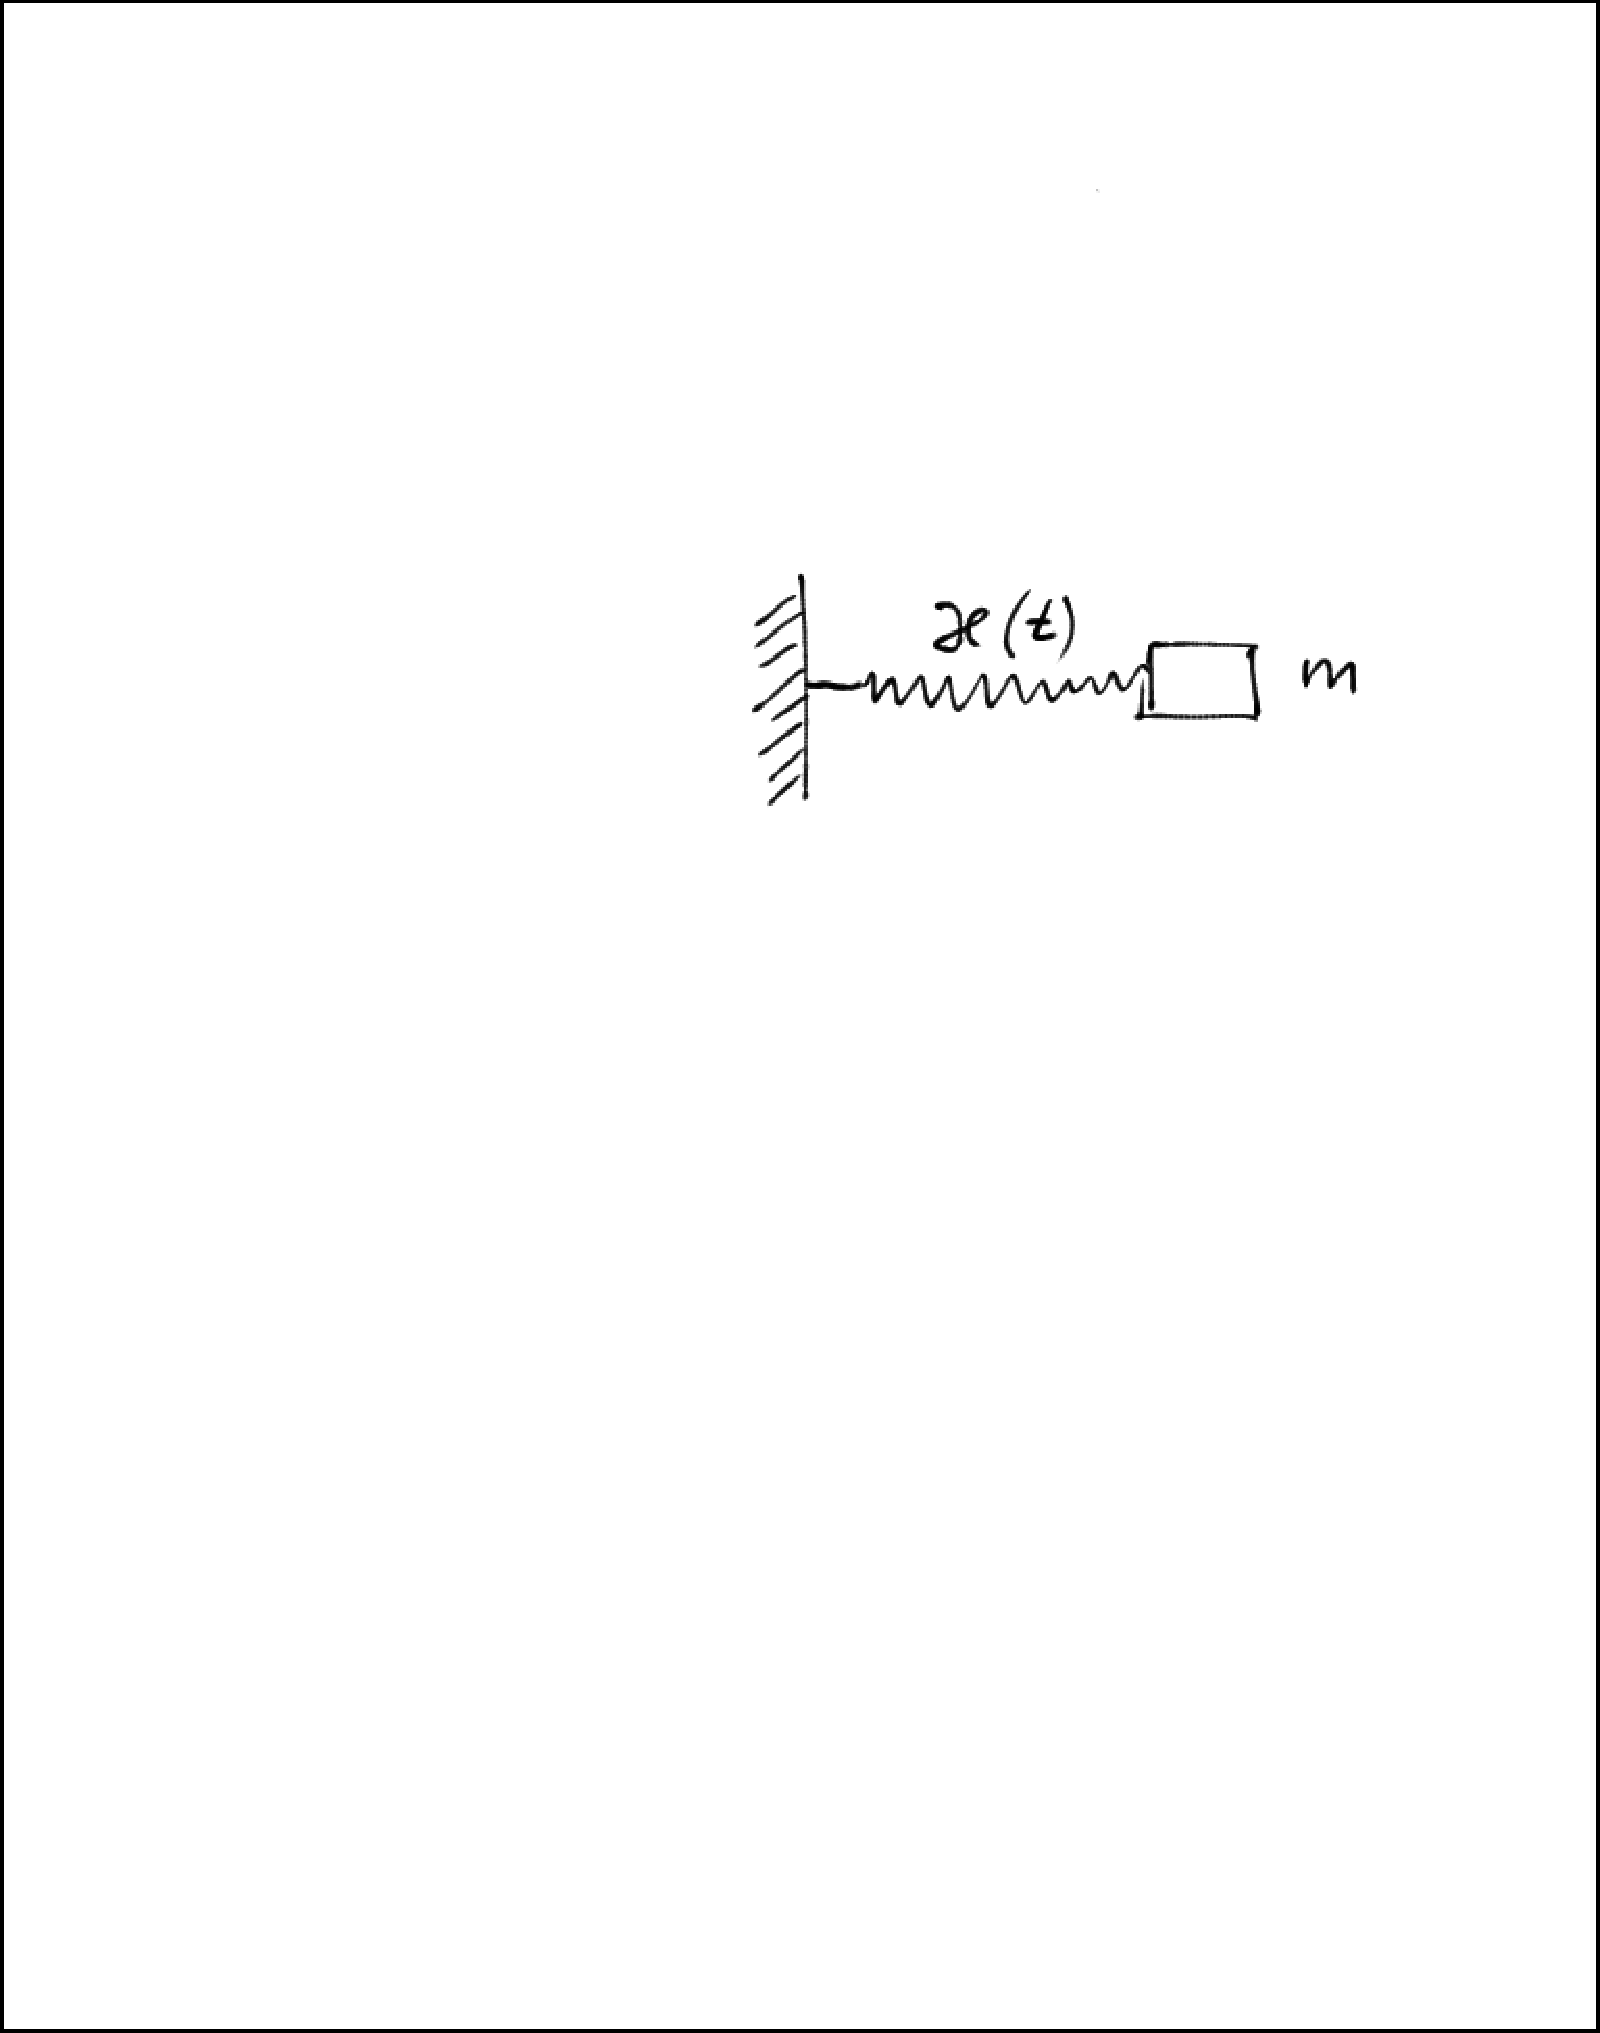
\includegraphics[scale=0.4]{pic5.png}}
\end{figure}
\begin{gather*}
\dv{E}{t} = \pdv{U(tx)}{t} = \pdv{U}{\varkappa} \dv{\varkappa}{t} = \frac{\Dot{\varkappa} x^2}{2},\\
\expval{\dv{E}{t}} =  \expval{\frac{\Dot{\varkappa}x^2}{2}},\\
 U = \frac{\varkappa x^2}{2}, \text{при этом} \expval{\frac{\varkappa x^2}{2}} = \frac{\varkappa}{2} \expval{x^2}, \text{так как } \tau_T \gg \tau_0, \text{то есть $\varkappa(t)$ меняется сильно медленнее, а}\\
\expval{U} = \frac{1}{2} \expval{E} \text{по теореме о вириале},\\
\expval{\dv{E}{t}} \eqq{\bf{?}} \dv{t}\expval{E} = \frac{\dot{\varkappa}}{\varkappa} \expval{U} = \frac{\dot{\varkappa}}{2 \varkappa} \expval{E} \Rightarrow\\
\dv{t} \ln{\expval{E}} = \frac{1}{2} \dv{t} \ln{\varkappa} = \dv{t} \ln{\sqrt{\varkappa}} \Rightarrow\\
\expval{E} = E_0 \sqrt{\frac{\varkappa(t)}{\varkappa_0}} \Rightarrow\\
\boxed{\frac{\expval{E}}{\omega(t)} \simeq const}
\end{gather*}
\end{ex}

\begin{thm}[Теорема о вириале для системы частиц]
\end{thm}
\begin{proof}
Аналогично тому, как это было проделано в доказательстве теоремы о вириале дя одной материальной точки, получим следующее утверждение:
\begin{equation}
\expval{T} \approx -\frac{1}{2} \sum\limits_{i=1}^N \vb{F}_i \vb{r}_i, \text{сумма в правой части --- вириал Клаузиуса.}
\end{equation}
\begin{gather*}
\vb{F}_i^{(e)} = - \pdv{\vb{r}}U^{(e)},\\
\vb{F}_{ij}^{(i)} = -\pdv{U_{ij}^{(i)}}{\vb{r}_i} = \pdv{U_{ij}}{\rho_{ij}},\\
\sum\limits_{i=1}^{3N} \vb{F}_i^{(e)} \vb{r}_i = -\sum\limits_{i=1}^N \pdv{U^{(e)}}{\vb{r}_i} \vb{r}_i = -k^{(e)} U^{(e)},\\
\sum\limits_{\substack{i=1\\ i \neq j}}^{N} \vb{F}_{ij}^{(i)} \vb{r}_i = -\sum\limits_{i \neq j} \frac{1}{2} \pdv{U^{(i)}_{ij}}{\vb*{\rho}_{ij}} \vb*{\rho}_{ij} = -k^{(i)} U^{(i)}\\
\boxed{\expval{T} = \frac{k^{(i)}}{2} \expval{U^{(i)}} + \frac{k^{(e)}}{2} \expval{U^{(e)}}}\\
E = T + U^{(i)} + U^{(e)}
\end{gather*}
\end{proof}
\newpage
\begin{ex}[Твёрдое тело]
$$\vb*{\rho}_{ij} = const \Rightarrow U^{(i)} = const, k^{(i)} = 0$$
$$\boxed{\expval{T} = \frac{k^{(e)}}{2} \expval{U^{(e)}}}$$
\end{ex}

\begin{ex}[Эргодическая гипотеза]
$\mathstrut$\\
\begin{figure}[h!]\centering
\def\svgwidth{5cm}
\input{ergodic.pdf_tex}
\end{figure}
\begin{gather*}
\expval{T} =   -\hlf \expval{\sum_i \vb{F}_i \vb{r}_i} = \frac{p}{2} \int\limits_{S_V} \vb{r} \dd{\vb{S}} = \frac{3}{2} pV\\
\vb{F}_i = -p \dd{\vb{S}_i}, U_i^{(i)} = 0\\
\oint \vb{r} \dd{\vb{S}} = \int\limits_0^{2\pi} \int\limits_0^\pi aa^2 \sin\theta \dd{\theta} = 4\pi a^3 = 3V \\
\div\vb{r} = \pdv{x_i}{x_i} \Rightarrow \oint \vb{r} \dd{\vb{S}} = \int \div\vb{r} \dd{V} = 3 \int \dd{V} = 3V.
\end{gather*}
\end{ex}

\begin{ex}[Термодинамическое равновесие в звезде]
Пусть теперь внешних сил нет --- только внутренние. Рассмотрим две звезды одной плотности, но отличающиеся по размерам в два раза. Какая из них горячее?
\begin{multicols}{3}
\begin{gather*}
U^{(e)} = 0,\\
U^{(i)}_{ij} = -\frac{\alpha}{\rho_{ij}} \Rightarrow k^{(i)} = -1,\\
 \expval{T} = - \hlf \expval{U^{(i)}},
\end{gather*}
\begin{gather*}
\expval{T} = \frac{3}{2}k_\text{Б} \frac{m}{\mu} T_\star,\\
\expval{U^{(i)}} = -G \frac{m^2}{R} \Rightarrow\\
\end{gather*}
\begin{gather*}
T_\star \sim \frac{m}{R} \sim R^2 \rho.
\end{gather*}
\end{multicols}
\end{ex}
\newpage
